\documentclass[twoside]{book}

% Packages required by doxygen
\usepackage{fixltx2e}
\usepackage{calc}
\usepackage{doxygen}
\usepackage[export]{adjustbox} % also loads graphicx
\usepackage{graphicx}
\usepackage[utf8]{inputenc}
\usepackage{makeidx}
\usepackage{multicol}
\usepackage{multirow}
\PassOptionsToPackage{warn}{textcomp}
\usepackage{textcomp}
\usepackage[nointegrals]{wasysym}
\usepackage[table]{xcolor}

% Font selection
\usepackage[T1]{fontenc}
\usepackage[scaled=.90]{helvet}
\usepackage{courier}
\usepackage{amssymb}
\usepackage{sectsty}
\renewcommand{\familydefault}{\sfdefault}
\allsectionsfont{%
  \fontseries{bc}\selectfont%
  \color{darkgray}%
}
\renewcommand{\DoxyLabelFont}{%
  \fontseries{bc}\selectfont%
  \color{darkgray}%
}
\newcommand{\+}{\discretionary{\mbox{\scriptsize$\hookleftarrow$}}{}{}}

% Page & text layout
\usepackage{geometry}
\geometry{%
  a4paper,%
  top=2.5cm,%
  bottom=2.5cm,%
  left=2.5cm,%
  right=2.5cm%
}
\tolerance=750
\hfuzz=15pt
\hbadness=750
\setlength{\emergencystretch}{15pt}
\setlength{\parindent}{0cm}
\setlength{\parskip}{3ex plus 2ex minus 2ex}
\makeatletter
\renewcommand{\paragraph}{%
  \@startsection{paragraph}{4}{0ex}{-1.0ex}{1.0ex}{%
    \normalfont\normalsize\bfseries\SS@parafont%
  }%
}
\renewcommand{\subparagraph}{%
  \@startsection{subparagraph}{5}{0ex}{-1.0ex}{1.0ex}{%
    \normalfont\normalsize\bfseries\SS@subparafont%
  }%
}
\makeatother

% Headers & footers
\usepackage{fancyhdr}
\pagestyle{fancyplain}
\fancyhead[LE]{\fancyplain{}{\bfseries\thepage}}
\fancyhead[CE]{\fancyplain{}{}}
\fancyhead[RE]{\fancyplain{}{\bfseries\leftmark}}
\fancyhead[LO]{\fancyplain{}{\bfseries\rightmark}}
\fancyhead[CO]{\fancyplain{}{}}
\fancyhead[RO]{\fancyplain{}{\bfseries\thepage}}
\fancyfoot[LE]{\fancyplain{}{}}
\fancyfoot[CE]{\fancyplain{}{}}
\fancyfoot[RE]{\fancyplain{}{\bfseries\scriptsize Generated by Doxygen }}
\fancyfoot[LO]{\fancyplain{}{\bfseries\scriptsize Generated by Doxygen }}
\fancyfoot[CO]{\fancyplain{}{}}
\fancyfoot[RO]{\fancyplain{}{}}
\renewcommand{\footrulewidth}{0.4pt}
\renewcommand{\chaptermark}[1]{%
  \markboth{#1}{}%
}
\renewcommand{\sectionmark}[1]{%
  \markright{\thesection\ #1}%
}

% Indices & bibliography
\usepackage{natbib}
\usepackage[titles]{tocloft}
\setcounter{tocdepth}{3}
\setcounter{secnumdepth}{5}
\makeindex

% Hyperlinks (required, but should be loaded last)
\usepackage{ifpdf}
\ifpdf
  \usepackage[pdftex,pagebackref=true]{hyperref}
\else
  \usepackage[ps2pdf,pagebackref=true]{hyperref}
\fi
\hypersetup{%
  colorlinks=true,%
  linkcolor=blue,%
  citecolor=blue,%
  unicode%
}

% Custom commands
\newcommand{\clearemptydoublepage}{%
  \newpage{\pagestyle{empty}\cleardoublepage}%
}

\usepackage{caption}
\captionsetup{labelsep=space,justification=centering,font={bf},singlelinecheck=off,skip=4pt,position=top}

%===== C O N T E N T S =====

\begin{document}

% Titlepage & ToC
\hypersetup{pageanchor=false,
             bookmarksnumbered=true,
             pdfencoding=unicode
            }
\pagenumbering{alph}
\begin{titlepage}
\vspace*{7cm}
\begin{center}%
{\Large Decentralized Dummy \\[1ex]\large 1 }\\
\vspace*{1cm}
{\large Generated by Doxygen 1.8.13}\\
\end{center}
\end{titlepage}
\clearemptydoublepage
\pagenumbering{roman}
\tableofcontents
\clearemptydoublepage
\pagenumbering{arabic}
\hypersetup{pageanchor=true}

%--- Begin generated contents ---
\chapter{Class Index}
\section{Class List}
Here are the classes, structs, unions and interfaces with brief descriptions\+:\begin{DoxyCompactList}
\item\contentsline{section}{\hyperlink{structEXMPLE__s}{E\+X\+M\+P\+L\+E\+\_\+s} }{\pageref{structEXMPLE__s}}{}
\item\contentsline{section}{\hyperlink{classfile}{file} \\*File class for handling file access }{\pageref{classfile}}{}
\item\contentsline{section}{\hyperlink{classJSON__manager}{J\+S\+O\+N\+\_\+manager} \\*J\+S\+ON manager class for reading and parsing J\+S\+ON data }{\pageref{classJSON__manager}}{}
\item\contentsline{section}{\hyperlink{structUMGR__s}{U\+M\+G\+R\+\_\+s} \\*Struct which is specified to hold the values of the Update\+Manager U\+M\+GR }{\pageref{structUMGR__s}}{}
\end{DoxyCompactList}

\chapter{File Index}
\section{File List}
Here is a list of all files with brief descriptions\+:\begin{DoxyCompactList}
\item\contentsline{section}{/home/visxim/\+C\+Lion\+Projects/\+Decentralized\+Dummy\+Process/\hyperlink{file_8cpp}{file.\+cpp} }{\pageref{file_8cpp}}{}
\item\contentsline{section}{/home/visxim/\+C\+Lion\+Projects/\+Decentralized\+Dummy\+Process/\hyperlink{JSON__manager_8cpp}{J\+S\+O\+N\+\_\+manager.\+cpp} \\*J\+S\+O\+N\+\_\+manager for handling J\+S\+ON data }{\pageref{JSON__manager_8cpp}}{}
\item\contentsline{section}{/home/visxim/\+C\+Lion\+Projects/\+Decentralized\+Dummy\+Process/\hyperlink{main_8cpp}{main.\+cpp} \\*Main of the decentralized dummy process }{\pageref{main_8cpp}}{}
\item\contentsline{section}{/home/visxim/\+C\+Lion\+Projects/\+Decentralized\+Dummy\+Process/\hyperlink{time-tp_8c}{time-\/tp.\+c} }{\pageref{time-tp_8c}}{}
\end{DoxyCompactList}

\chapter{Class Documentation}
\input{structEXMPLE__s}
\hypertarget{classfile}{}\section{file Class Reference}
\label{classfile}\index{file@{file}}


File class for handling file access.  




{\ttfamily \#include $<$file.\+h$>$}



Collaboration diagram for file\+:
\nopagebreak
\begin{figure}[H]
\begin{center}
\leavevmode
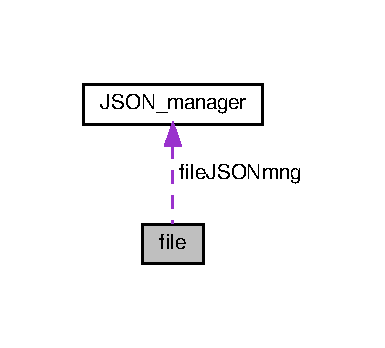
\includegraphics[width=185pt]{classfile__coll__graph}
\end{center}
\end{figure}
\subsection*{Public Member Functions}
\begin{DoxyCompactItemize}
\item 
void \hyperlink{classfile_a04d228a8eabeb75ed6f6f7c87f5053db}{setfilename} (string \hyperlink{classfile}{file})
\begin{DoxyCompactList}\small\item\em Function for setting the filename of the configuration file for this file-\/object. \end{DoxyCompactList}\item 
void \hyperlink{classfile_a6f3aeac1f4b08cd52b7879ea999fded1}{call\+J\+S\+ON} ()
\begin{DoxyCompactList}\small\item\em Function for retreiving the J\+S\+ON information from the file. \end{DoxyCompactList}\end{DoxyCompactItemize}
\subsection*{Public Attributes}
\begin{DoxyCompactItemize}
\item 
\hyperlink{classJSON__manager}{J\+S\+O\+N\+\_\+manager} \hyperlink{classfile_aaba2c5a6566d9cbbc9fb613475eb1ce7}{file\+J\+S\+O\+Nmng}
\end{DoxyCompactItemize}
\subsection*{Private Attributes}
\begin{DoxyCompactItemize}
\item 
string \hyperlink{classfile_a9117ee5ddda3538f631fe96252de70fc}{filename}
\end{DoxyCompactItemize}


\subsection{Detailed Description}
File class for handling file access. 

\subsection{Member Function Documentation}
\mbox{\Hypertarget{classfile_a6f3aeac1f4b08cd52b7879ea999fded1}\label{classfile_a6f3aeac1f4b08cd52b7879ea999fded1}} 
\index{file@{file}!call\+J\+S\+ON@{call\+J\+S\+ON}}
\index{call\+J\+S\+ON@{call\+J\+S\+ON}!file@{file}}
\subsubsection{\texorpdfstring{call\+J\+S\+O\+N()}{callJSON()}}
{\footnotesize\ttfamily void file\+::call\+J\+S\+ON (\begin{DoxyParamCaption}{ }\end{DoxyParamCaption})}



Function for retreiving the J\+S\+ON information from the file. 

Here is the call graph for this function\+:
\nopagebreak
\begin{figure}[H]
\begin{center}
\leavevmode
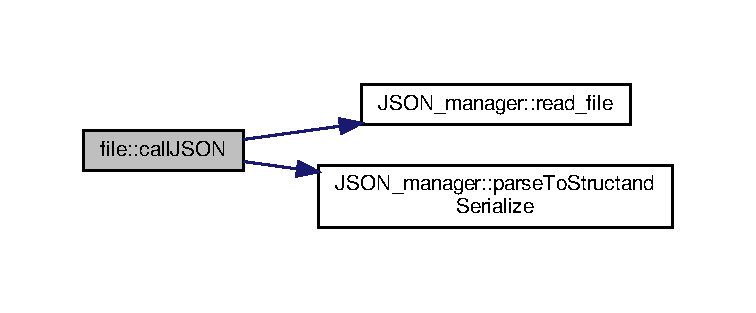
\includegraphics[width=350pt]{classfile_a6f3aeac1f4b08cd52b7879ea999fded1_cgraph}
\end{center}
\end{figure}
\mbox{\Hypertarget{classfile_a04d228a8eabeb75ed6f6f7c87f5053db}\label{classfile_a04d228a8eabeb75ed6f6f7c87f5053db}} 
\index{file@{file}!setfilename@{setfilename}}
\index{setfilename@{setfilename}!file@{file}}
\subsubsection{\texorpdfstring{setfilename()}{setfilename()}}
{\footnotesize\ttfamily void file\+::setfilename (\begin{DoxyParamCaption}\item[{string}]{file }\end{DoxyParamCaption})}



Function for setting the filename of the configuration file for this file-\/object. 



\subsection{Member Data Documentation}
\mbox{\Hypertarget{classfile_aaba2c5a6566d9cbbc9fb613475eb1ce7}\label{classfile_aaba2c5a6566d9cbbc9fb613475eb1ce7}} 
\index{file@{file}!file\+J\+S\+O\+Nmng@{file\+J\+S\+O\+Nmng}}
\index{file\+J\+S\+O\+Nmng@{file\+J\+S\+O\+Nmng}!file@{file}}
\subsubsection{\texorpdfstring{file\+J\+S\+O\+Nmng}{fileJSONmng}}
{\footnotesize\ttfamily \hyperlink{classJSON__manager}{J\+S\+O\+N\+\_\+manager} file\+::file\+J\+S\+O\+Nmng}

\mbox{\Hypertarget{classfile_a9117ee5ddda3538f631fe96252de70fc}\label{classfile_a9117ee5ddda3538f631fe96252de70fc}} 
\index{file@{file}!filename@{filename}}
\index{filename@{filename}!file@{file}}
\subsubsection{\texorpdfstring{filename}{filename}}
{\footnotesize\ttfamily string file\+::filename\hspace{0.3cm}{\ttfamily [private]}}



The documentation for this class was generated from the following files\+:\begin{DoxyCompactItemize}
\item 
/home/visxim/\+C\+Lion\+Projects/\+Decentralized\+Dummy\+Process/includes/\hyperlink{file_8h}{file.\+h}\item 
/home/visxim/\+C\+Lion\+Projects/\+Decentralized\+Dummy\+Process/\hyperlink{file_8cpp}{file.\+cpp}\end{DoxyCompactItemize}

\hypertarget{classJSON__manager}{}\section{J\+S\+O\+N\+\_\+manager Class Reference}
\label{classJSON__manager}\index{J\+S\+O\+N\+\_\+manager@{J\+S\+O\+N\+\_\+manager}}


J\+S\+ON manager class for reading and parsing J\+S\+ON data.  




{\ttfamily \#include $<$J\+S\+O\+N\+\_\+manager.\+h$>$}

\subsection*{Public Member Functions}
\begin{DoxyCompactItemize}
\item 
unsigned int \hyperlink{classJSON__manager_a9b600a34d73fd3f28bf00ddf3f2e6640}{read\+\_\+file} (string filename)
\begin{DoxyCompactList}\small\item\em Function for reading the J\+S\+ON file and parsing it into a document object. \end{DoxyCompactList}\item 
string \hyperlink{classJSON__manager_a5d05e5f8eb6883f38181d48cf26cc5fc}{get\+\_\+json\+\_\+config\+\_\+string} ()
\begin{DoxyCompactList}\small\item\em Return the whole J\+S\+ON data as a string from the document object. \end{DoxyCompactList}\item 
unsigned int \hyperlink{classJSON__manager_a7bb6db218d195494ca939233671cb183}{parse\+To\+Structand\+Serialize} (string filename)
\begin{DoxyCompactList}\small\item\em Function for parsing the interpreted J\+S\+ON data from the file into a predefinied struct (to find in \hyperlink{data__storage_8h}{data\+\_\+storage.\+h}) \end{DoxyCompactList}\end{DoxyCompactItemize}
\subsection*{Private Attributes}
\begin{DoxyCompactItemize}
\item 
Document \hyperlink{classJSON__manager_afa1c5569b74bd68fe785d553c798c4dd}{doc}
\end{DoxyCompactItemize}


\subsection{Detailed Description}
J\+S\+ON manager class for reading and parsing J\+S\+ON data. 

\subsection{Member Function Documentation}
\mbox{\Hypertarget{classJSON__manager_a5d05e5f8eb6883f38181d48cf26cc5fc}\label{classJSON__manager_a5d05e5f8eb6883f38181d48cf26cc5fc}} 
\index{J\+S\+O\+N\+\_\+manager@{J\+S\+O\+N\+\_\+manager}!get\+\_\+json\+\_\+config\+\_\+string@{get\+\_\+json\+\_\+config\+\_\+string}}
\index{get\+\_\+json\+\_\+config\+\_\+string@{get\+\_\+json\+\_\+config\+\_\+string}!J\+S\+O\+N\+\_\+manager@{J\+S\+O\+N\+\_\+manager}}
\subsubsection{\texorpdfstring{get\+\_\+json\+\_\+config\+\_\+string()}{get\_json\_config\_string()}}
{\footnotesize\ttfamily string J\+S\+O\+N\+\_\+manager\+::get\+\_\+json\+\_\+config\+\_\+string (\begin{DoxyParamCaption}{ }\end{DoxyParamCaption})}



Return the whole J\+S\+ON data as a string from the document object. 

\mbox{\Hypertarget{classJSON__manager_a7bb6db218d195494ca939233671cb183}\label{classJSON__manager_a7bb6db218d195494ca939233671cb183}} 
\index{J\+S\+O\+N\+\_\+manager@{J\+S\+O\+N\+\_\+manager}!parse\+To\+Structand\+Serialize@{parse\+To\+Structand\+Serialize}}
\index{parse\+To\+Structand\+Serialize@{parse\+To\+Structand\+Serialize}!J\+S\+O\+N\+\_\+manager@{J\+S\+O\+N\+\_\+manager}}
\subsubsection{\texorpdfstring{parse\+To\+Structand\+Serialize()}{parseToStructandSerialize()}}
{\footnotesize\ttfamily unsigned int J\+S\+O\+N\+\_\+manager\+::parse\+To\+Structand\+Serialize (\begin{DoxyParamCaption}\item[{string}]{filename }\end{DoxyParamCaption})}



Function for parsing the interpreted J\+S\+ON data from the file into a predefinied struct (to find in \hyperlink{data__storage_8h}{data\+\_\+storage.\+h}) 

compare the filename to find the right implementation

create the matching struct

parse all the data into this struct

compare the filename to find the right implementation

create the matching struct

parse all the data into this struct

default case \mbox{\Hypertarget{classJSON__manager_a9b600a34d73fd3f28bf00ddf3f2e6640}\label{classJSON__manager_a9b600a34d73fd3f28bf00ddf3f2e6640}} 
\index{J\+S\+O\+N\+\_\+manager@{J\+S\+O\+N\+\_\+manager}!read\+\_\+file@{read\+\_\+file}}
\index{read\+\_\+file@{read\+\_\+file}!J\+S\+O\+N\+\_\+manager@{J\+S\+O\+N\+\_\+manager}}
\subsubsection{\texorpdfstring{read\+\_\+file()}{read\_file()}}
{\footnotesize\ttfamily unsigned int J\+S\+O\+N\+\_\+manager\+::read\+\_\+file (\begin{DoxyParamCaption}\item[{string}]{filename }\end{DoxyParamCaption})}



Function for reading the J\+S\+ON file and parsing it into a document object. 

Read the whole file line by line and store it into the \char`\"{}json\char`\"{} string

convert the read string into const char$\ast$ and parse to document

Parse the converted \char`\"{}json\char`\"{} string into a document object 

\subsection{Member Data Documentation}
\mbox{\Hypertarget{classJSON__manager_afa1c5569b74bd68fe785d553c798c4dd}\label{classJSON__manager_afa1c5569b74bd68fe785d553c798c4dd}} 
\index{J\+S\+O\+N\+\_\+manager@{J\+S\+O\+N\+\_\+manager}!doc@{doc}}
\index{doc@{doc}!J\+S\+O\+N\+\_\+manager@{J\+S\+O\+N\+\_\+manager}}
\subsubsection{\texorpdfstring{doc}{doc}}
{\footnotesize\ttfamily Document J\+S\+O\+N\+\_\+manager\+::doc\hspace{0.3cm}{\ttfamily [private]}}



The documentation for this class was generated from the following files\+:\begin{DoxyCompactItemize}
\item 
/home/visxim/\+C\+Lion\+Projects/\+Decentralized\+Dummy\+Process/includes/\hyperlink{JSON__manager_8h}{J\+S\+O\+N\+\_\+manager.\+h}\item 
/home/visxim/\+C\+Lion\+Projects/\+Decentralized\+Dummy\+Process/\hyperlink{JSON__manager_8cpp}{J\+S\+O\+N\+\_\+manager.\+cpp}\end{DoxyCompactItemize}

\hypertarget{structUMGR__s}{}\section{U\+M\+G\+R\+\_\+s Struct Reference}
\label{structUMGR__s}\index{U\+M\+G\+R\+\_\+s@{U\+M\+G\+R\+\_\+s}}


Struct which is specified to hold the values of the Update\+Manager U\+M\+GR.  




{\ttfamily \#include $<$data\+\_\+storage.\+h$>$}

\subsection*{Public Member Functions}
\begin{DoxyCompactItemize}
\item 
{\footnotesize template$<$typename Archive $>$ }\\void \hyperlink{structUMGR__s_af85ccf0554e33a7f7163c0d26ca791eb}{serialize} (Archive \&ar, const unsigned int version)
\begin{DoxyCompactList}\small\item\em function for serializing the struct \end{DoxyCompactList}\end{DoxyCompactItemize}
\subsection*{Public Attributes}
\begin{DoxyCompactItemize}
\item 
string \hyperlink{structUMGR__s_a3d36ca5f936e211da7645b00894c68dd}{name}
\item 
string \hyperlink{structUMGR__s_a80540aaa70f1333ba3c558f6af7a39a1}{description}
\item 
string \hyperlink{structUMGR__s_a0a329d092b37dd9061136642d6bebd15}{dlt\+\_\+id}
\item 
string \hyperlink{structUMGR__s_ab9ebb2767a511f0e791ae1f07b2a03e2}{log\+\_\+mode}
\item 
string \hyperlink{structUMGR__s_a59eaa08e65bbab14ab1deb4969a261c3}{log\+\_\+level}
\item 
string \hyperlink{structUMGR__s_ae8d842a1050f74d35c2785f9d72f7197}{log\+\_\+dir\+\_\+path}
\item 
unsigned int \hyperlink{structUMGR__s_a9024c1140605de70cf368de635024702}{ipc\+\_\+port}
\item 
unsigned int \hyperlink{structUMGR__s_af846433f5bfd716a224c3cf7ac208fdb}{reconnection\+\_\+retry\+\_\+offset}
\item 
unsigned int \hyperlink{structUMGR__s_aa3ce6d48e8db2d85e084d079548b8338}{msg\+\_\+buf\+\_\+size}
\item 
int \hyperlink{structUMGR__s_a3a98cb14c2b8c9545aa47871865076e6}{checksum}
\end{DoxyCompactItemize}


\subsection{Detailed Description}
Struct which is specified to hold the values of the Update\+Manager U\+M\+GR. 

\subsection{Member Function Documentation}
\mbox{\Hypertarget{structUMGR__s_af85ccf0554e33a7f7163c0d26ca791eb}\label{structUMGR__s_af85ccf0554e33a7f7163c0d26ca791eb}} 
\index{U\+M\+G\+R\+\_\+s@{U\+M\+G\+R\+\_\+s}!serialize@{serialize}}
\index{serialize@{serialize}!U\+M\+G\+R\+\_\+s@{U\+M\+G\+R\+\_\+s}}
\subsubsection{\texorpdfstring{serialize()}{serialize()}}
{\footnotesize\ttfamily template$<$typename Archive $>$ \\
void U\+M\+G\+R\+\_\+s\+::serialize (\begin{DoxyParamCaption}\item[{Archive \&}]{ar,  }\item[{const unsigned int}]{version }\end{DoxyParamCaption})\hspace{0.3cm}{\ttfamily [inline]}}



function for serializing the struct 



\subsection{Member Data Documentation}
\mbox{\Hypertarget{structUMGR__s_a3a98cb14c2b8c9545aa47871865076e6}\label{structUMGR__s_a3a98cb14c2b8c9545aa47871865076e6}} 
\index{U\+M\+G\+R\+\_\+s@{U\+M\+G\+R\+\_\+s}!checksum@{checksum}}
\index{checksum@{checksum}!U\+M\+G\+R\+\_\+s@{U\+M\+G\+R\+\_\+s}}
\subsubsection{\texorpdfstring{checksum}{checksum}}
{\footnotesize\ttfamily int U\+M\+G\+R\+\_\+s\+::checksum}

\mbox{\Hypertarget{structUMGR__s_a80540aaa70f1333ba3c558f6af7a39a1}\label{structUMGR__s_a80540aaa70f1333ba3c558f6af7a39a1}} 
\index{U\+M\+G\+R\+\_\+s@{U\+M\+G\+R\+\_\+s}!description@{description}}
\index{description@{description}!U\+M\+G\+R\+\_\+s@{U\+M\+G\+R\+\_\+s}}
\subsubsection{\texorpdfstring{description}{description}}
{\footnotesize\ttfamily string U\+M\+G\+R\+\_\+s\+::description}

\mbox{\Hypertarget{structUMGR__s_a0a329d092b37dd9061136642d6bebd15}\label{structUMGR__s_a0a329d092b37dd9061136642d6bebd15}} 
\index{U\+M\+G\+R\+\_\+s@{U\+M\+G\+R\+\_\+s}!dlt\+\_\+id@{dlt\+\_\+id}}
\index{dlt\+\_\+id@{dlt\+\_\+id}!U\+M\+G\+R\+\_\+s@{U\+M\+G\+R\+\_\+s}}
\subsubsection{\texorpdfstring{dlt\+\_\+id}{dlt\_id}}
{\footnotesize\ttfamily string U\+M\+G\+R\+\_\+s\+::dlt\+\_\+id}

\mbox{\Hypertarget{structUMGR__s_a9024c1140605de70cf368de635024702}\label{structUMGR__s_a9024c1140605de70cf368de635024702}} 
\index{U\+M\+G\+R\+\_\+s@{U\+M\+G\+R\+\_\+s}!ipc\+\_\+port@{ipc\+\_\+port}}
\index{ipc\+\_\+port@{ipc\+\_\+port}!U\+M\+G\+R\+\_\+s@{U\+M\+G\+R\+\_\+s}}
\subsubsection{\texorpdfstring{ipc\+\_\+port}{ipc\_port}}
{\footnotesize\ttfamily unsigned int U\+M\+G\+R\+\_\+s\+::ipc\+\_\+port}

\mbox{\Hypertarget{structUMGR__s_ae8d842a1050f74d35c2785f9d72f7197}\label{structUMGR__s_ae8d842a1050f74d35c2785f9d72f7197}} 
\index{U\+M\+G\+R\+\_\+s@{U\+M\+G\+R\+\_\+s}!log\+\_\+dir\+\_\+path@{log\+\_\+dir\+\_\+path}}
\index{log\+\_\+dir\+\_\+path@{log\+\_\+dir\+\_\+path}!U\+M\+G\+R\+\_\+s@{U\+M\+G\+R\+\_\+s}}
\subsubsection{\texorpdfstring{log\+\_\+dir\+\_\+path}{log\_dir\_path}}
{\footnotesize\ttfamily string U\+M\+G\+R\+\_\+s\+::log\+\_\+dir\+\_\+path}

\mbox{\Hypertarget{structUMGR__s_a59eaa08e65bbab14ab1deb4969a261c3}\label{structUMGR__s_a59eaa08e65bbab14ab1deb4969a261c3}} 
\index{U\+M\+G\+R\+\_\+s@{U\+M\+G\+R\+\_\+s}!log\+\_\+level@{log\+\_\+level}}
\index{log\+\_\+level@{log\+\_\+level}!U\+M\+G\+R\+\_\+s@{U\+M\+G\+R\+\_\+s}}
\subsubsection{\texorpdfstring{log\+\_\+level}{log\_level}}
{\footnotesize\ttfamily string U\+M\+G\+R\+\_\+s\+::log\+\_\+level}

\mbox{\Hypertarget{structUMGR__s_ab9ebb2767a511f0e791ae1f07b2a03e2}\label{structUMGR__s_ab9ebb2767a511f0e791ae1f07b2a03e2}} 
\index{U\+M\+G\+R\+\_\+s@{U\+M\+G\+R\+\_\+s}!log\+\_\+mode@{log\+\_\+mode}}
\index{log\+\_\+mode@{log\+\_\+mode}!U\+M\+G\+R\+\_\+s@{U\+M\+G\+R\+\_\+s}}
\subsubsection{\texorpdfstring{log\+\_\+mode}{log\_mode}}
{\footnotesize\ttfamily string U\+M\+G\+R\+\_\+s\+::log\+\_\+mode}

\mbox{\Hypertarget{structUMGR__s_aa3ce6d48e8db2d85e084d079548b8338}\label{structUMGR__s_aa3ce6d48e8db2d85e084d079548b8338}} 
\index{U\+M\+G\+R\+\_\+s@{U\+M\+G\+R\+\_\+s}!msg\+\_\+buf\+\_\+size@{msg\+\_\+buf\+\_\+size}}
\index{msg\+\_\+buf\+\_\+size@{msg\+\_\+buf\+\_\+size}!U\+M\+G\+R\+\_\+s@{U\+M\+G\+R\+\_\+s}}
\subsubsection{\texorpdfstring{msg\+\_\+buf\+\_\+size}{msg\_buf\_size}}
{\footnotesize\ttfamily unsigned int U\+M\+G\+R\+\_\+s\+::msg\+\_\+buf\+\_\+size}

\mbox{\Hypertarget{structUMGR__s_a3d36ca5f936e211da7645b00894c68dd}\label{structUMGR__s_a3d36ca5f936e211da7645b00894c68dd}} 
\index{U\+M\+G\+R\+\_\+s@{U\+M\+G\+R\+\_\+s}!name@{name}}
\index{name@{name}!U\+M\+G\+R\+\_\+s@{U\+M\+G\+R\+\_\+s}}
\subsubsection{\texorpdfstring{name}{name}}
{\footnotesize\ttfamily string U\+M\+G\+R\+\_\+s\+::name}

\mbox{\Hypertarget{structUMGR__s_af846433f5bfd716a224c3cf7ac208fdb}\label{structUMGR__s_af846433f5bfd716a224c3cf7ac208fdb}} 
\index{U\+M\+G\+R\+\_\+s@{U\+M\+G\+R\+\_\+s}!reconnection\+\_\+retry\+\_\+offset@{reconnection\+\_\+retry\+\_\+offset}}
\index{reconnection\+\_\+retry\+\_\+offset@{reconnection\+\_\+retry\+\_\+offset}!U\+M\+G\+R\+\_\+s@{U\+M\+G\+R\+\_\+s}}
\subsubsection{\texorpdfstring{reconnection\+\_\+retry\+\_\+offset}{reconnection\_retry\_offset}}
{\footnotesize\ttfamily unsigned int U\+M\+G\+R\+\_\+s\+::reconnection\+\_\+retry\+\_\+offset}



The documentation for this struct was generated from the following file\+:\begin{DoxyCompactItemize}
\item 
/home/visxim/\+C\+Lion\+Projects/\+Decentralized\+Dummy\+Process/includes/\hyperlink{data__storage_8h}{data\+\_\+storage.\+h}\end{DoxyCompactItemize}

\chapter{File Documentation}
\hypertarget{file_8cpp}{}\section{/home/visxim/\+C\+Lion\+Projects/\+Decentralized\+Dummy\+Process/file.cpp File Reference}
\label{file_8cpp}\index{/home/visxim/\+C\+Lion\+Projects/\+Decentralized\+Dummy\+Process/file.\+cpp@{/home/visxim/\+C\+Lion\+Projects/\+Decentralized\+Dummy\+Process/file.\+cpp}}
{\ttfamily \#include \char`\"{}file.\+h\char`\"{}}\newline
Include dependency graph for file.\+cpp\+:
\nopagebreak
\begin{figure}[H]
\begin{center}
\leavevmode
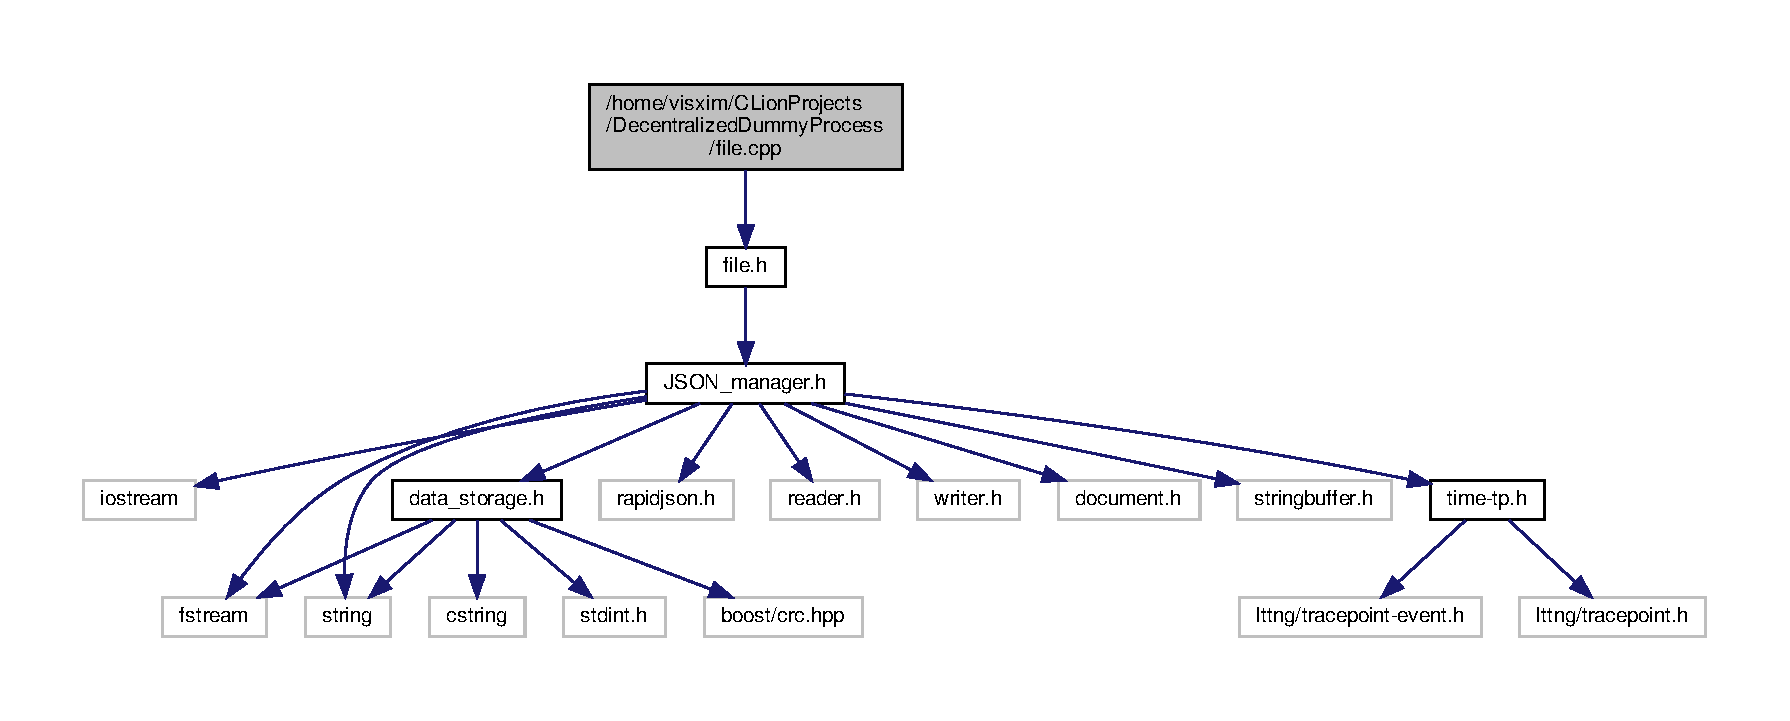
\includegraphics[width=350pt]{file_8cpp__incl}
\end{center}
\end{figure}

\hypertarget{data__storage_8h}{}\section{/home/visxim/\+C\+Lion\+Projects/\+Decentralized\+Dummy\+Process/includes/data\+\_\+storage.h File Reference}
\label{data__storage_8h}\index{/home/visxim/\+C\+Lion\+Projects/\+Decentralized\+Dummy\+Process/includes/data\+\_\+storage.\+h@{/home/visxim/\+C\+Lion\+Projects/\+Decentralized\+Dummy\+Process/includes/data\+\_\+storage.\+h}}


Header of checksum\+\_\+manager for checking the integrity of the data.  


{\ttfamily \#include $<$fstream$>$}\newline
{\ttfamily \#include $<$string$>$}\newline
{\ttfamily \#include $<$cstring$>$}\newline
{\ttfamily \#include $<$stdint.\+h$>$}\newline
{\ttfamily \#include \char`\"{}boost/crc.\+hpp\char`\"{}}\newline
Include dependency graph for data\+\_\+storage.\+h\+:
\nopagebreak
\begin{figure}[H]
\begin{center}
\leavevmode
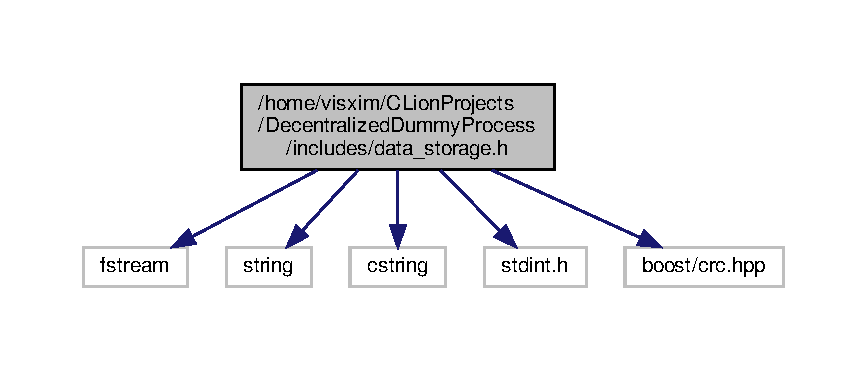
\includegraphics[width=350pt]{data__storage_8h__incl}
\end{center}
\end{figure}
This graph shows which files directly or indirectly include this file\+:
\nopagebreak
\begin{figure}[H]
\begin{center}
\leavevmode
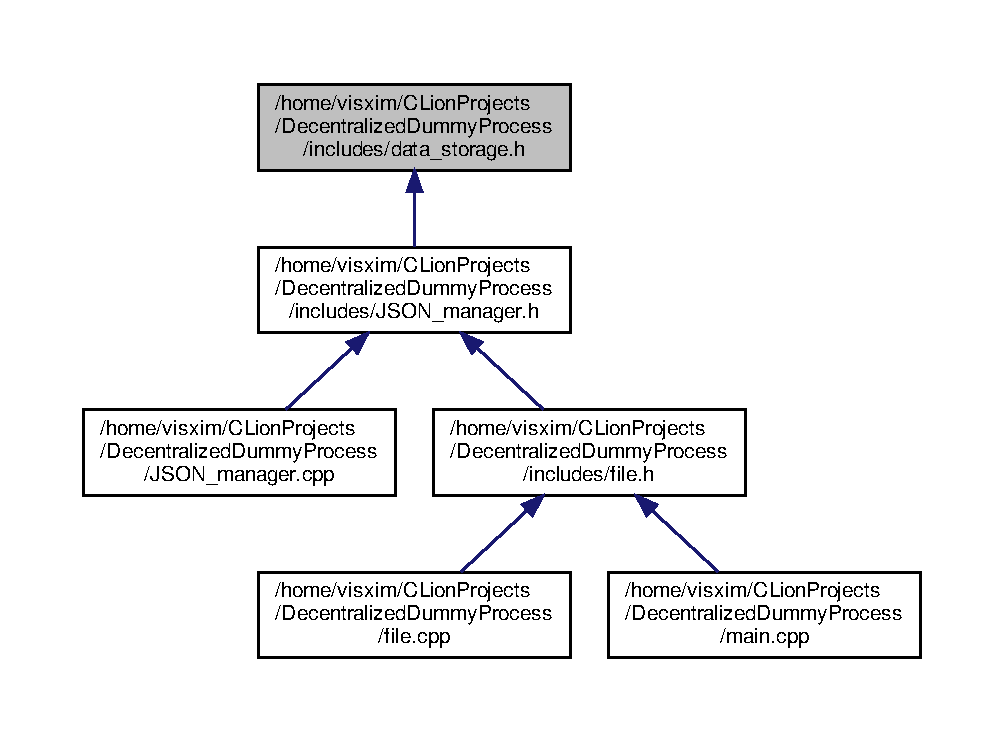
\includegraphics[width=350pt]{data__storage_8h__dep__incl}
\end{center}
\end{figure}
\subsection*{Classes}
\begin{DoxyCompactItemize}
\item 
struct \hyperlink{structUMGR__s}{U\+M\+G\+R\+\_\+s}
\begin{DoxyCompactList}\small\item\em Struct which is specified to hold the values of the Update\+Manager U\+M\+GR. \end{DoxyCompactList}\item 
struct \hyperlink{structEXMPLE__s}{E\+X\+M\+P\+L\+E\+\_\+s}
\end{DoxyCompactItemize}


\subsection{Detailed Description}
Header of checksum\+\_\+manager for checking the integrity of the data. 

The Checksum\+\_\+manager creates and checks if the data is valid 
\hypertarget{file_8h}{}\section{/home/visxim/\+C\+Lion\+Projects/\+Decentralized\+Dummy\+Process/includes/file.h File Reference}
\label{file_8h}\index{/home/visxim/\+C\+Lion\+Projects/\+Decentralized\+Dummy\+Process/includes/file.\+h@{/home/visxim/\+C\+Lion\+Projects/\+Decentralized\+Dummy\+Process/includes/file.\+h}}


Header of file methods for file handling.  


{\ttfamily \#include \char`\"{}J\+S\+O\+N\+\_\+manager.\+h\char`\"{}}\newline
Include dependency graph for file.\+h\+:
\nopagebreak
\begin{figure}[H]
\begin{center}
\leavevmode
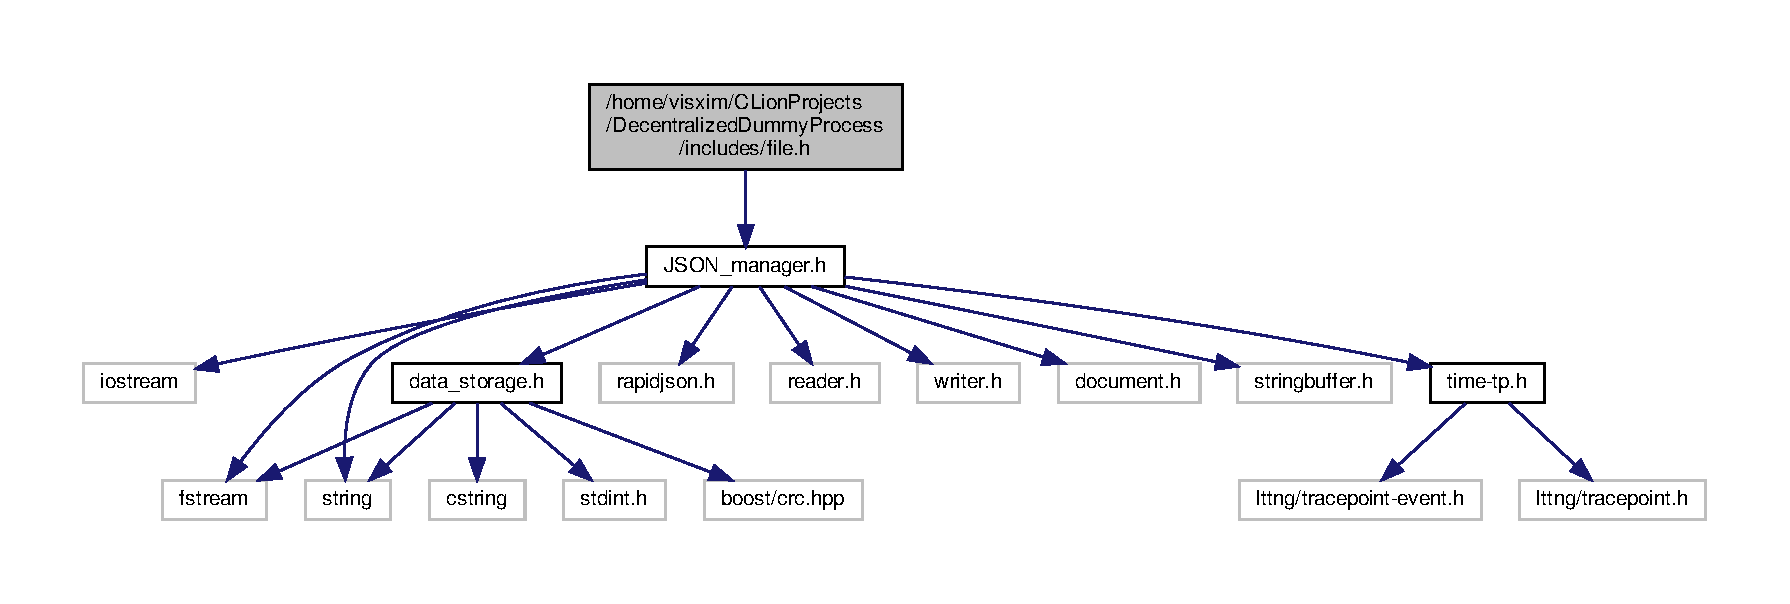
\includegraphics[width=350pt]{file_8h__incl}
\end{center}
\end{figure}
This graph shows which files directly or indirectly include this file\+:
\nopagebreak
\begin{figure}[H]
\begin{center}
\leavevmode
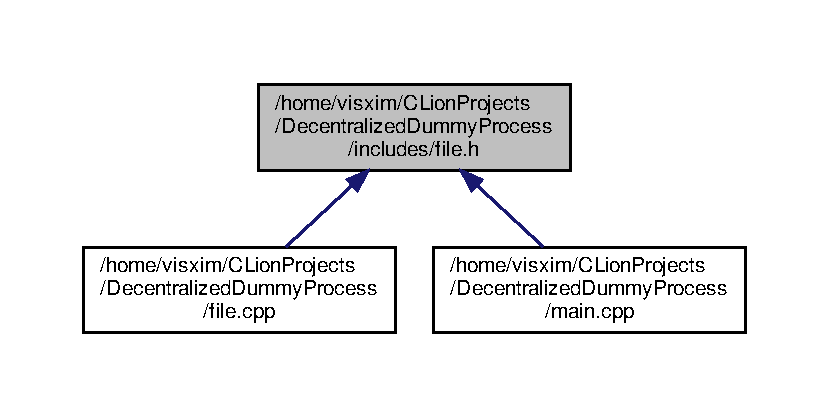
\includegraphics[width=350pt]{file_8h__dep__incl}
\end{center}
\end{figure}
\subsection*{Classes}
\begin{DoxyCompactItemize}
\item 
class \hyperlink{classfile}{file}
\begin{DoxyCompactList}\small\item\em File class for handling file access. \end{DoxyCompactList}\end{DoxyCompactItemize}


\subsection{Detailed Description}
Header of file methods for file handling. 

The file is for accessing the files with the configurations 
\hypertarget{JSON__manager_8h}{}\section{/home/visxim/\+C\+Lion\+Projects/\+Decentralized\+Dummy\+Process/includes/\+J\+S\+O\+N\+\_\+manager.h File Reference}
\label{JSON__manager_8h}\index{/home/visxim/\+C\+Lion\+Projects/\+Decentralized\+Dummy\+Process/includes/\+J\+S\+O\+N\+\_\+manager.\+h@{/home/visxim/\+C\+Lion\+Projects/\+Decentralized\+Dummy\+Process/includes/\+J\+S\+O\+N\+\_\+manager.\+h}}


Header of \hyperlink{classJSON__manager}{J\+S\+O\+N\+\_\+manager} for handling J\+S\+ON data.  


{\ttfamily \#include $<$iostream$>$}\newline
{\ttfamily \#include $<$fstream$>$}\newline
{\ttfamily \#include $<$string$>$}\newline
{\ttfamily \#include \char`\"{}rapidjson.\+h\char`\"{}}\newline
{\ttfamily \#include \char`\"{}reader.\+h\char`\"{}}\newline
{\ttfamily \#include \char`\"{}writer.\+h\char`\"{}}\newline
{\ttfamily \#include \char`\"{}document.\+h\char`\"{}}\newline
{\ttfamily \#include \char`\"{}stringbuffer.\+h\char`\"{}}\newline
{\ttfamily \#include \char`\"{}data\+\_\+storage.\+h\char`\"{}}\newline
{\ttfamily \#include \char`\"{}time-\/tp.\+h\char`\"{}}\newline
Include dependency graph for J\+S\+O\+N\+\_\+manager.\+h\+:
\nopagebreak
\begin{figure}[H]
\begin{center}
\leavevmode
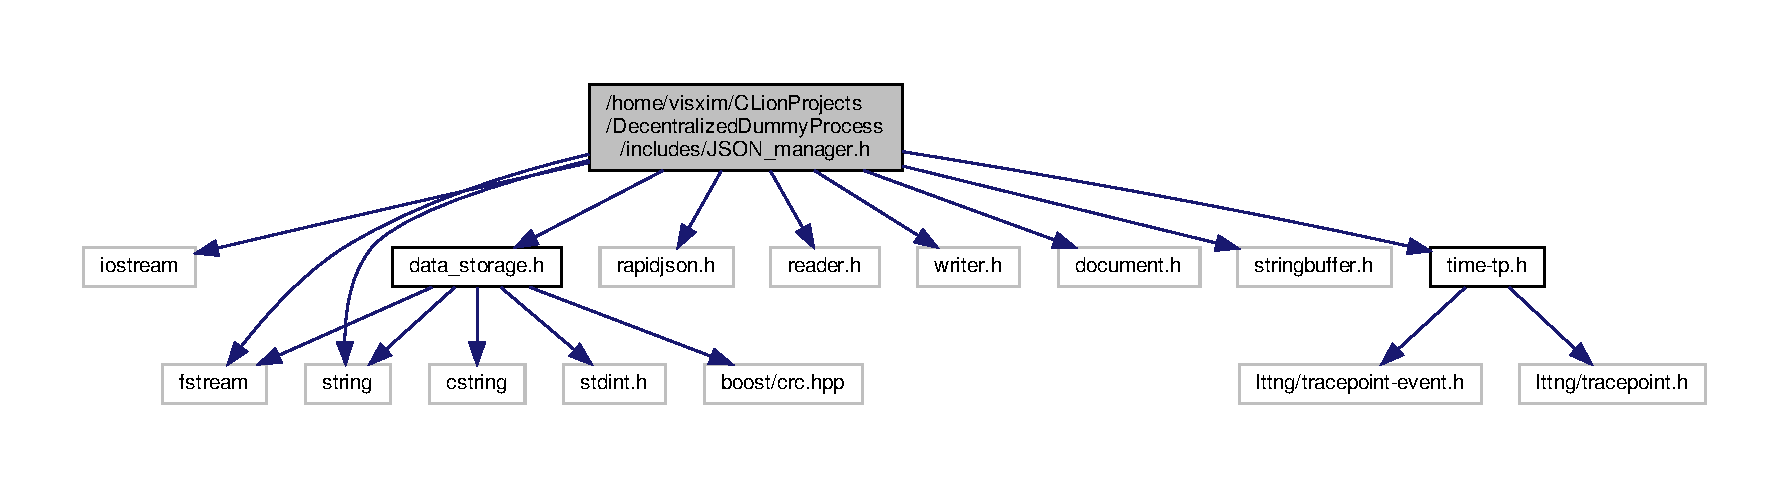
\includegraphics[width=350pt]{JSON__manager_8h__incl}
\end{center}
\end{figure}
This graph shows which files directly or indirectly include this file\+:
\nopagebreak
\begin{figure}[H]
\begin{center}
\leavevmode
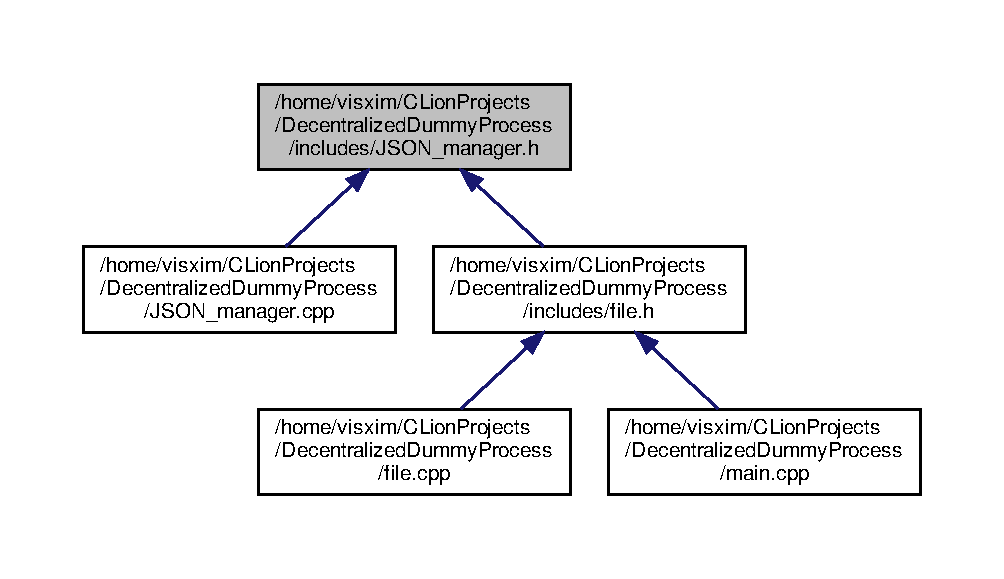
\includegraphics[width=350pt]{JSON__manager_8h__dep__incl}
\end{center}
\end{figure}
\subsection*{Classes}
\begin{DoxyCompactItemize}
\item 
class \hyperlink{classJSON__manager}{J\+S\+O\+N\+\_\+manager}
\begin{DoxyCompactList}\small\item\em J\+S\+ON manager class for reading and parsing J\+S\+ON data. \end{DoxyCompactList}\end{DoxyCompactItemize}


\subsection{Detailed Description}
Header of \hyperlink{classJSON__manager}{J\+S\+O\+N\+\_\+manager} for handling J\+S\+ON data. 

The \hyperlink{classJSON__manager}{J\+S\+O\+N\+\_\+manager} handels the interpretation and storage of the J\+S\+ON data from the given file 
\hypertarget{time-tp_8h}{}\section{/home/visxim/\+C\+Lion\+Projects/\+Decentralized\+Dummy\+Process/includes/time-\/tp.h File Reference}
\label{time-tp_8h}\index{/home/visxim/\+C\+Lion\+Projects/\+Decentralized\+Dummy\+Process/includes/time-\/tp.\+h@{/home/visxim/\+C\+Lion\+Projects/\+Decentralized\+Dummy\+Process/includes/time-\/tp.\+h}}
{\ttfamily \#include $<$lttng/tracepoint.\+h$>$}\newline
{\ttfamily \#include $<$lttng/tracepoint-\/event.\+h$>$}\newline
Include dependency graph for time-\/tp.h\+:
\nopagebreak
\begin{figure}[H]
\begin{center}
\leavevmode
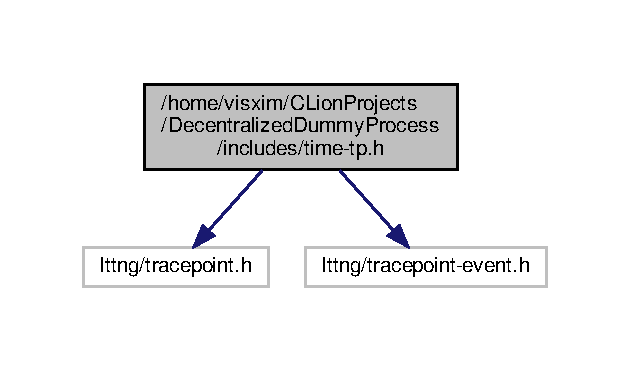
\includegraphics[width=303pt]{time-tp_8h__incl}
\end{center}
\end{figure}
This graph shows which files directly or indirectly include this file\+:
\nopagebreak
\begin{figure}[H]
\begin{center}
\leavevmode
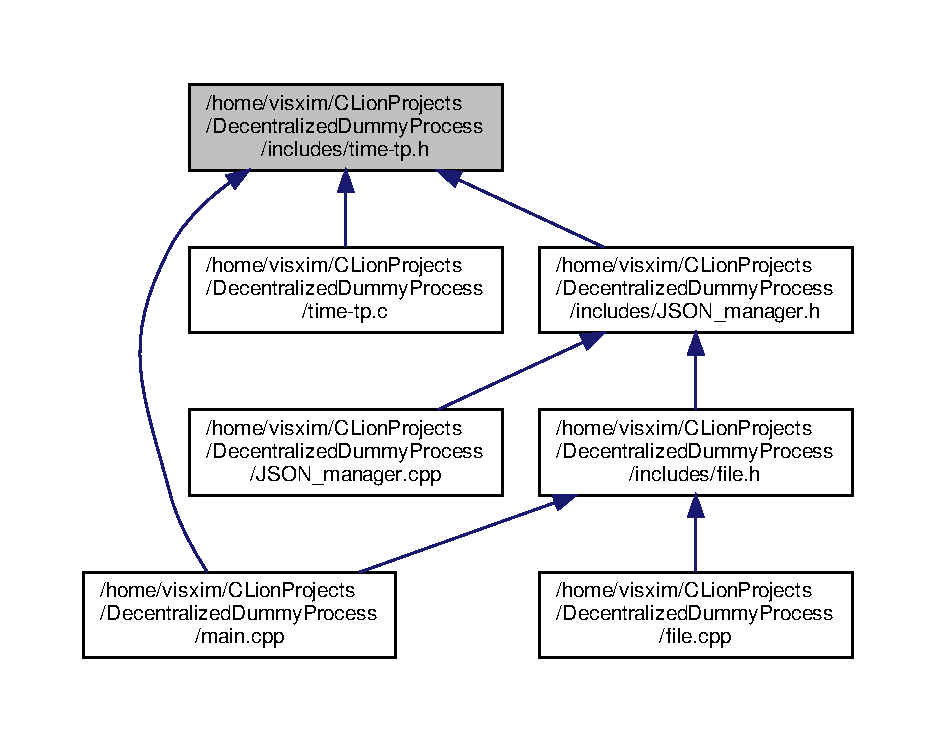
\includegraphics[width=350pt]{time-tp_8h__dep__incl}
\end{center}
\end{figure}
\subsection*{Macros}
\begin{DoxyCompactItemize}
\item 
\#define \hyperlink{time-tp_8h_a6751837690af3a0ad19fb209a69dd16e}{T\+R\+A\+C\+E\+P\+O\+I\+N\+T\+\_\+\+P\+R\+O\+V\+I\+D\+ER}~tp\+\_\+provider
\item 
\#define \hyperlink{time-tp_8h_a090261faa16d05fb6993d61861ba8ff9}{T\+R\+A\+C\+E\+P\+O\+I\+N\+T\+\_\+\+I\+N\+C\+L\+U\+DE}~\char`\"{}./time-\/tp.\+h\char`\"{}
\item 
\#define \hyperlink{time-tp_8h_ad91ef7d5cc408393bcfaf376512d4ce7}{\+\_\+time\+\_\+\+T\+P\+\_\+H}
\end{DoxyCompactItemize}
\subsection*{Functions}
\begin{DoxyCompactItemize}
\item 
\hyperlink{time-tp_8h_ae23da3516b0a9868651c7da43c8d6a61}{T\+R\+A\+C\+E\+P\+O\+I\+N\+T\+\_\+\+E\+V\+E\+NT} (tp\+\_\+provider, time\+\_\+tracepoint, \hyperlink{time-tp_8h_a369ab506413cfc785534f5fb47faa636}{T\+P\+\_\+\+A\+R\+GS}(int, probe\+\_\+nr), T\+P\+\_\+\+F\+I\+E\+L\+DS(ctf\+\_\+integer(int, probe\+Number, probe\+\_\+nr))) T\+R\+A\+C\+E\+P\+O\+I\+N\+T\+\_\+\+E\+V\+E\+NT(tp\+\_\+provider
\item 
\hyperlink{time-tp_8h_a369ab506413cfc785534f5fb47faa636}{T\+P\+\_\+\+A\+R\+GS} ()
\end{DoxyCompactItemize}
\subsection*{Variables}
\begin{DoxyCompactItemize}
\item 
\hyperlink{time-tp_8h_ab28129dca0cec2a82e678cd4c60216dc}{overall\+\_\+time\+\_\+tracepoint}
\end{DoxyCompactItemize}


\subsection{Macro Definition Documentation}
\mbox{\Hypertarget{time-tp_8h_ad91ef7d5cc408393bcfaf376512d4ce7}\label{time-tp_8h_ad91ef7d5cc408393bcfaf376512d4ce7}} 
\index{time-\/tp.\+h@{time-\/tp.\+h}!\+\_\+time\+\_\+\+T\+P\+\_\+H@{\+\_\+time\+\_\+\+T\+P\+\_\+H}}
\index{\+\_\+time\+\_\+\+T\+P\+\_\+H@{\+\_\+time\+\_\+\+T\+P\+\_\+H}!time-\/tp.\+h@{time-\/tp.\+h}}
\subsubsection{\texorpdfstring{\+\_\+time\+\_\+\+T\+P\+\_\+H}{\_time\_TP\_H}}
{\footnotesize\ttfamily \#define \+\_\+time\+\_\+\+T\+P\+\_\+H}

\mbox{\Hypertarget{time-tp_8h_a090261faa16d05fb6993d61861ba8ff9}\label{time-tp_8h_a090261faa16d05fb6993d61861ba8ff9}} 
\index{time-\/tp.\+h@{time-\/tp.\+h}!T\+R\+A\+C\+E\+P\+O\+I\+N\+T\+\_\+\+I\+N\+C\+L\+U\+DE@{T\+R\+A\+C\+E\+P\+O\+I\+N\+T\+\_\+\+I\+N\+C\+L\+U\+DE}}
\index{T\+R\+A\+C\+E\+P\+O\+I\+N\+T\+\_\+\+I\+N\+C\+L\+U\+DE@{T\+R\+A\+C\+E\+P\+O\+I\+N\+T\+\_\+\+I\+N\+C\+L\+U\+DE}!time-\/tp.\+h@{time-\/tp.\+h}}
\subsubsection{\texorpdfstring{T\+R\+A\+C\+E\+P\+O\+I\+N\+T\+\_\+\+I\+N\+C\+L\+U\+DE}{TRACEPOINT\_INCLUDE}}
{\footnotesize\ttfamily \#define T\+R\+A\+C\+E\+P\+O\+I\+N\+T\+\_\+\+I\+N\+C\+L\+U\+DE~\char`\"{}./time-\/tp.\+h\char`\"{}}

\mbox{\Hypertarget{time-tp_8h_a6751837690af3a0ad19fb209a69dd16e}\label{time-tp_8h_a6751837690af3a0ad19fb209a69dd16e}} 
\index{time-\/tp.\+h@{time-\/tp.\+h}!T\+R\+A\+C\+E\+P\+O\+I\+N\+T\+\_\+\+P\+R\+O\+V\+I\+D\+ER@{T\+R\+A\+C\+E\+P\+O\+I\+N\+T\+\_\+\+P\+R\+O\+V\+I\+D\+ER}}
\index{T\+R\+A\+C\+E\+P\+O\+I\+N\+T\+\_\+\+P\+R\+O\+V\+I\+D\+ER@{T\+R\+A\+C\+E\+P\+O\+I\+N\+T\+\_\+\+P\+R\+O\+V\+I\+D\+ER}!time-\/tp.\+h@{time-\/tp.\+h}}
\subsubsection{\texorpdfstring{T\+R\+A\+C\+E\+P\+O\+I\+N\+T\+\_\+\+P\+R\+O\+V\+I\+D\+ER}{TRACEPOINT\_PROVIDER}}
{\footnotesize\ttfamily \#define T\+R\+A\+C\+E\+P\+O\+I\+N\+T\+\_\+\+P\+R\+O\+V\+I\+D\+ER~tp\+\_\+provider}



\subsection{Function Documentation}
\mbox{\Hypertarget{time-tp_8h_a369ab506413cfc785534f5fb47faa636}\label{time-tp_8h_a369ab506413cfc785534f5fb47faa636}} 
\index{time-\/tp.\+h@{time-\/tp.\+h}!T\+P\+\_\+\+A\+R\+GS@{T\+P\+\_\+\+A\+R\+GS}}
\index{T\+P\+\_\+\+A\+R\+GS@{T\+P\+\_\+\+A\+R\+GS}!time-\/tp.\+h@{time-\/tp.\+h}}
\subsubsection{\texorpdfstring{T\+P\+\_\+\+A\+R\+G\+S()}{TP\_ARGS()}}
{\footnotesize\ttfamily T\+P\+\_\+\+A\+R\+GS (\begin{DoxyParamCaption}{ }\end{DoxyParamCaption})}

\mbox{\Hypertarget{time-tp_8h_ae23da3516b0a9868651c7da43c8d6a61}\label{time-tp_8h_ae23da3516b0a9868651c7da43c8d6a61}} 
\index{time-\/tp.\+h@{time-\/tp.\+h}!T\+R\+A\+C\+E\+P\+O\+I\+N\+T\+\_\+\+E\+V\+E\+NT@{T\+R\+A\+C\+E\+P\+O\+I\+N\+T\+\_\+\+E\+V\+E\+NT}}
\index{T\+R\+A\+C\+E\+P\+O\+I\+N\+T\+\_\+\+E\+V\+E\+NT@{T\+R\+A\+C\+E\+P\+O\+I\+N\+T\+\_\+\+E\+V\+E\+NT}!time-\/tp.\+h@{time-\/tp.\+h}}
\subsubsection{\texorpdfstring{T\+R\+A\+C\+E\+P\+O\+I\+N\+T\+\_\+\+E\+V\+E\+N\+T()}{TRACEPOINT\_EVENT()}}
{\footnotesize\ttfamily T\+R\+A\+C\+E\+P\+O\+I\+N\+T\+\_\+\+E\+V\+E\+NT (\begin{DoxyParamCaption}\item[{tp\+\_\+provider}]{,  }\item[{time\+\_\+tracepoint}]{,  }\item[{\hyperlink{time-tp_8h_a369ab506413cfc785534f5fb47faa636}{T\+P\+\_\+\+A\+R\+GS}( int, probe\+\_\+nr)}]{,  }\item[{T\+P\+\_\+\+F\+I\+E\+L\+DS( ctf\+\_\+integer(int, probe\+Number, probe\+\_\+nr))}]{ }\end{DoxyParamCaption})}



\subsection{Variable Documentation}
\mbox{\Hypertarget{time-tp_8h_ab28129dca0cec2a82e678cd4c60216dc}\label{time-tp_8h_ab28129dca0cec2a82e678cd4c60216dc}} 
\index{time-\/tp.\+h@{time-\/tp.\+h}!overall\+\_\+time\+\_\+tracepoint@{overall\+\_\+time\+\_\+tracepoint}}
\index{overall\+\_\+time\+\_\+tracepoint@{overall\+\_\+time\+\_\+tracepoint}!time-\/tp.\+h@{time-\/tp.\+h}}
\subsubsection{\texorpdfstring{overall\+\_\+time\+\_\+tracepoint}{overall\_time\_tracepoint}}
{\footnotesize\ttfamily overall\+\_\+time\+\_\+tracepoint}


\hypertarget{JSON__manager_8cpp}{}\section{/home/visxim/\+C\+Lion\+Projects/\+Decentralized\+Dummy\+Process/\+J\+S\+O\+N\+\_\+manager.cpp File Reference}
\label{JSON__manager_8cpp}\index{/home/visxim/\+C\+Lion\+Projects/\+Decentralized\+Dummy\+Process/\+J\+S\+O\+N\+\_\+manager.\+cpp@{/home/visxim/\+C\+Lion\+Projects/\+Decentralized\+Dummy\+Process/\+J\+S\+O\+N\+\_\+manager.\+cpp}}


J\+S\+O\+N\+\_\+manager for handling J\+S\+ON data.  


{\ttfamily \#include \char`\"{}J\+S\+O\+N\+\_\+manager.\+h\char`\"{}}\newline
Include dependency graph for J\+S\+O\+N\+\_\+manager.\+cpp\+:
\nopagebreak
\begin{figure}[H]
\begin{center}
\leavevmode
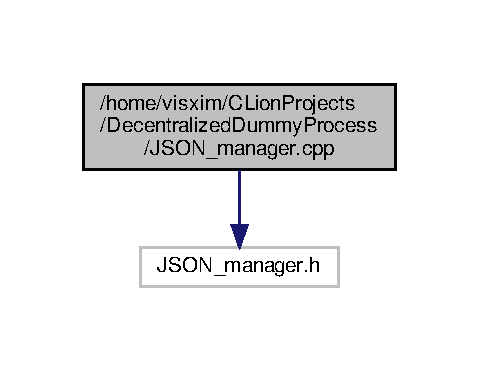
\includegraphics[width=230pt]{JSON__manager_8cpp__incl}
\end{center}
\end{figure}


\subsection{Detailed Description}
J\+S\+O\+N\+\_\+manager for handling J\+S\+ON data. 

The J\+S\+O\+N\+\_\+manager handels the interpretation and storage of the J\+S\+ON data from the given file 
\hypertarget{main_8cpp}{}\section{/home/visxim/\+C\+Lion\+Projects/\+Decentralized\+Dummy\+Process/main.cpp File Reference}
\label{main_8cpp}\index{/home/visxim/\+C\+Lion\+Projects/\+Decentralized\+Dummy\+Process/main.\+cpp@{/home/visxim/\+C\+Lion\+Projects/\+Decentralized\+Dummy\+Process/main.\+cpp}}


main of the decentralized dummy process  


{\ttfamily \#include \char`\"{}file.\+h\char`\"{}}\newline
{\ttfamily \#include \char`\"{}time-\/tp.\+h\char`\"{}}\newline
Include dependency graph for main.\+cpp\+:
\nopagebreak
\begin{figure}[H]
\begin{center}
\leavevmode
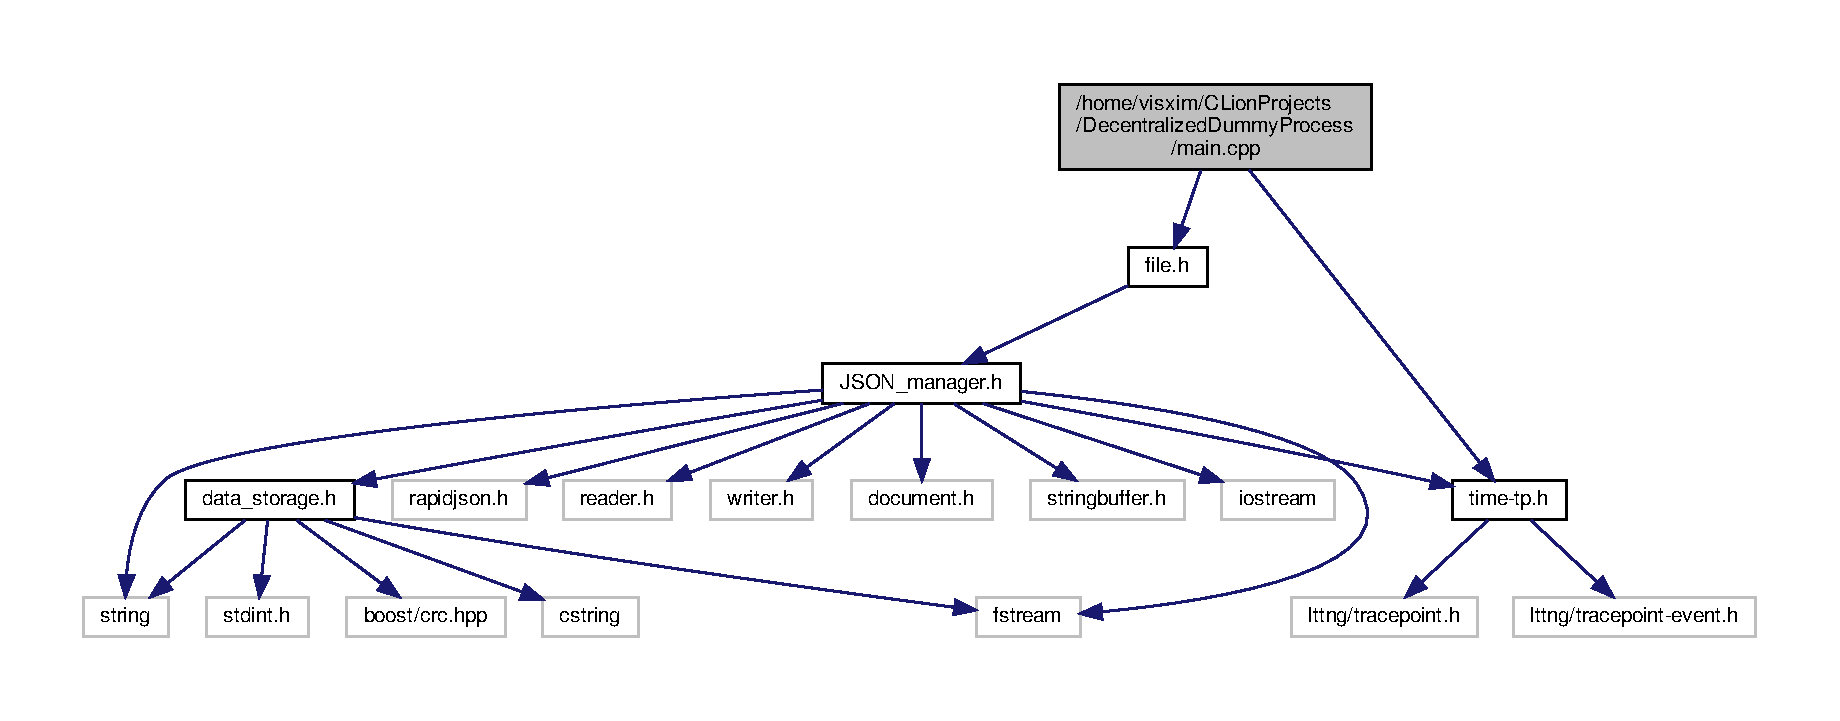
\includegraphics[width=350pt]{main_8cpp__incl}
\end{center}
\end{figure}
\subsection*{Functions}
\begin{DoxyCompactItemize}
\item 
int \hyperlink{main_8cpp_a3c04138a5bfe5d72780bb7e82a18e627}{main} (int argc, char $\ast$$\ast$argv)
\begin{DoxyCompactList}\small\item\em main function \end{DoxyCompactList}\end{DoxyCompactItemize}


\subsection{Detailed Description}
main of the decentralized dummy process 



\subsection{Function Documentation}
\mbox{\Hypertarget{main_8cpp_a3c04138a5bfe5d72780bb7e82a18e627}\label{main_8cpp_a3c04138a5bfe5d72780bb7e82a18e627}} 
\index{main.\+cpp@{main.\+cpp}!main@{main}}
\index{main@{main}!main.\+cpp@{main.\+cpp}}
\subsubsection{\texorpdfstring{main()}{main()}}
{\footnotesize\ttfamily int main (\begin{DoxyParamCaption}\item[{int}]{argc,  }\item[{char $\ast$$\ast$}]{argv }\end{DoxyParamCaption})}



main function 

Here is the call graph for this function\+:
\nopagebreak
\begin{figure}[H]
\begin{center}
\leavevmode
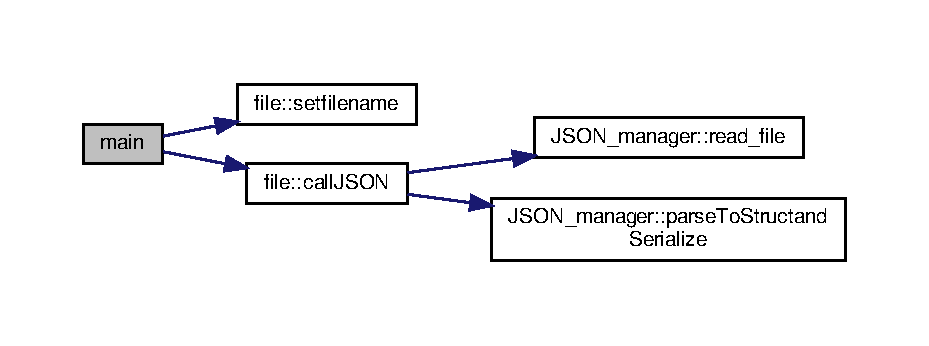
\includegraphics[width=350pt]{main_8cpp_a3c04138a5bfe5d72780bb7e82a18e627_cgraph}
\end{center}
\end{figure}

\hypertarget{time-tp_8c}{}\section{/home/visxim/\+C\+Lion\+Projects/\+Decentralized\+Dummy\+Process/time-\/tp.c File Reference}
\label{time-tp_8c}\index{/home/visxim/\+C\+Lion\+Projects/\+Decentralized\+Dummy\+Process/time-\/tp.\+c@{/home/visxim/\+C\+Lion\+Projects/\+Decentralized\+Dummy\+Process/time-\/tp.\+c}}
{\ttfamily \#include \char`\"{}time-\/tp.\+h\char`\"{}}\newline
Include dependency graph for time-\/tp.c\+:
\nopagebreak
\begin{figure}[H]
\begin{center}
\leavevmode
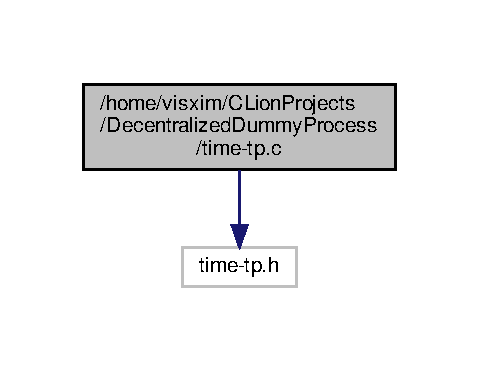
\includegraphics[width=230pt]{time-tp_8c__incl}
\end{center}
\end{figure}
\subsection*{Macros}
\begin{DoxyCompactItemize}
\item 
\#define \hyperlink{time-tp_8c_aeb980b4a64d9b54d660780a30415b0bc}{T\+R\+A\+C\+E\+P\+O\+I\+N\+T\+\_\+\+C\+R\+E\+A\+T\+E\+\_\+\+P\+R\+O\+B\+ES}
\item 
\#define \hyperlink{time-tp_8c_a71ad37c54f22eb10bdfed4267d53bd79}{T\+R\+A\+C\+E\+P\+O\+I\+N\+T\+\_\+\+D\+E\+F\+I\+NE}
\end{DoxyCompactItemize}


\subsection{Macro Definition Documentation}
\mbox{\Hypertarget{time-tp_8c_aeb980b4a64d9b54d660780a30415b0bc}\label{time-tp_8c_aeb980b4a64d9b54d660780a30415b0bc}} 
\index{time-\/tp.\+c@{time-\/tp.\+c}!T\+R\+A\+C\+E\+P\+O\+I\+N\+T\+\_\+\+C\+R\+E\+A\+T\+E\+\_\+\+P\+R\+O\+B\+ES@{T\+R\+A\+C\+E\+P\+O\+I\+N\+T\+\_\+\+C\+R\+E\+A\+T\+E\+\_\+\+P\+R\+O\+B\+ES}}
\index{T\+R\+A\+C\+E\+P\+O\+I\+N\+T\+\_\+\+C\+R\+E\+A\+T\+E\+\_\+\+P\+R\+O\+B\+ES@{T\+R\+A\+C\+E\+P\+O\+I\+N\+T\+\_\+\+C\+R\+E\+A\+T\+E\+\_\+\+P\+R\+O\+B\+ES}!time-\/tp.\+c@{time-\/tp.\+c}}
\subsubsection{\texorpdfstring{T\+R\+A\+C\+E\+P\+O\+I\+N\+T\+\_\+\+C\+R\+E\+A\+T\+E\+\_\+\+P\+R\+O\+B\+ES}{TRACEPOINT\_CREATE\_PROBES}}
{\footnotesize\ttfamily \#define T\+R\+A\+C\+E\+P\+O\+I\+N\+T\+\_\+\+C\+R\+E\+A\+T\+E\+\_\+\+P\+R\+O\+B\+ES}

\mbox{\Hypertarget{time-tp_8c_a71ad37c54f22eb10bdfed4267d53bd79}\label{time-tp_8c_a71ad37c54f22eb10bdfed4267d53bd79}} 
\index{time-\/tp.\+c@{time-\/tp.\+c}!T\+R\+A\+C\+E\+P\+O\+I\+N\+T\+\_\+\+D\+E\+F\+I\+NE@{T\+R\+A\+C\+E\+P\+O\+I\+N\+T\+\_\+\+D\+E\+F\+I\+NE}}
\index{T\+R\+A\+C\+E\+P\+O\+I\+N\+T\+\_\+\+D\+E\+F\+I\+NE@{T\+R\+A\+C\+E\+P\+O\+I\+N\+T\+\_\+\+D\+E\+F\+I\+NE}!time-\/tp.\+c@{time-\/tp.\+c}}
\subsubsection{\texorpdfstring{T\+R\+A\+C\+E\+P\+O\+I\+N\+T\+\_\+\+D\+E\+F\+I\+NE}{TRACEPOINT\_DEFINE}}
{\footnotesize\ttfamily \#define T\+R\+A\+C\+E\+P\+O\+I\+N\+T\+\_\+\+D\+E\+F\+I\+NE}


%--- End generated contents ---

% Index
\backmatter
\newpage
\phantomsection
\clearemptydoublepage
\addcontentsline{toc}{chapter}{Index}
\printindex

\end{document}
